\documentclass{beamer}

% Copyright 2010 Drow Ltd.
% 
% In principle, this file can be redistributed and/or modified under
% the terms of the GNU Public License, version 2.
% 
% However, this file is supposed to be a template to be modified
% for your own needs. For this reason, if you use this file as a
% template and not specifically distribute it as part of a another
% package/program, I grant the extra permission to freely copy and
% modify this file as you see fit and even to delete this copyright
% notice. 
\mode<presentation>
{
  \usetheme[titleline=true,
  alternativetitlepage=true,
  titlepagelogo=images/Java_logo]{Torino}
  \usecolortheme{nouvelle}
  \beamertemplatenavigationsymbolsempty
}

\usepackage{times}
\usepackage[utf8]{inputenc}
\usepackage[english,bulgarian]{babel}
\usepackage[T2A]{fontenc}

\usepackage{listings}
\lstset{language=Java,
  captionpos=b,
  tabsize=4,
  keywordstyle=\color{blue},
  commentstyle=\color{gray},
  stringstyle=\color{green},
  numbers=left,
  breaklines=true,
  showstringspaces=false,
  basicstyle=\ttfamily,
  emph={label},
  frame=shadowbox, 
  rulesepcolor=\color{blue},
  columns=fixed}

\title{Класове и обекти в Java}

\author{инж. Божидар ~Бацов}

\institute{Drow Ltd.}

\date{9.11.2010}

\subject{Talks}
% This is only inserted into the PDF information catalog. Can be left
% out. 

\begin{document}

\begin{frame}
  \titlepage
\end{frame}

\begin{frame}{Съдържание}
  \tableofcontents[pausesections]
\end{frame}

\section{Обектно-ориентирано програмиране}

\subsection{Какво е ООП?}

\begin{frame}{Обектно-ориентирано програмиране(ООП)}
  \transdissolve
  \begin{itemize}
  \item Какво е ООП? \pause
  \item Основния понятия в ООП
    \begin{itemize}
    \item клас - шаблон \pause
    \item обект - инстанция на шаблон \pause
      \begin{itemize}
      \item състояние(state) \pause
      \item поведение(behaviour)
      \end{itemize}
    \end{itemize}
  \end{itemize}
\end{frame}

\begin{frame}{Пример - Клас Човек}
  \begin{columns}
    \column{.5\textwidth}
    Клас Човек
    \begin{itemize}
    \item атрибути \pause
      \begin{itemize}
      \item име
      \item възраст 
      \item адрес
      \end{itemize}
    \item поведение \pause
      \begin{itemize}
      \item говори
      \item ходи
      \end{itemize}
    \end{itemize} \pause

    \column{.5\textwidth}
    Обект от клас Човек
    \begin{itemize}
    \item състояние \pause
      \begin{itemize}
      \item Божидар
      \item 33 
      \item Готам Сити
      \end{itemize}
    \item поведение \pause
      \begin{itemize}
      \item Кажи "аааа"
      \item Ходи в бат пещерата
      \end{itemize}
    \end{itemize}
  \end{columns}
\end{frame}

\subsection{Класове и обекти}
\begin{frame}{Основни понятия при класовете}
  \transdissolve
  \begin{itemize}
  \item Атрибути
    \begin{itemize}
    \item описват структурата на обектите \pause
    \item реализирани са чрез полета(instance fields) \pause
    \end{itemize}
  \item Поведение \pause
    \begin{itemize}
    \item реализирано чрез методи(instance methods) \pause
    \end{itemize}
  \item Капсулиране на състоянието  \pause
    \begin{itemize}
    \item достъпно само чрез методи
    \end{itemize}
  \item Класово състояние/поведение \pause
    \begin{itemize}
    \item статични полета и методи \pause
    \end{itemize}
  \item Наследяване
  \end{itemize}
\end{frame}

\begin{frame}{Основни понятия при обектите}
  \transdissolve
  \begin{itemize}
  \item Състояние \pause
    \begin{itemize}
    \item стойности за атрибутите \pause
    \end{itemize}
  \item Поведение \pause
    \begin{itemize}
    \item операции над състоянието \pause
    \end{itemize}
  \item Идентичност \pause
    \begin{itemize}
    \item каква информация определя два обекта като еднакви
    \end{itemize}
  \end{itemize}
\end{frame}

\begin{frame}{Отношения между класовете}
  \transdissolve
  \begin{itemize}
  \item Зависимост(coupling, dependency, uses-a) \pause
    \begin{itemize}
    \item класове използвани от класа \pause
    \end{itemize}
  \item Агрегация(has-a) \pause
    \begin{itemize}
    \item индикира че един обект съдържа други обекти \pause
    \end{itemize}
  \item Наследяване(is-a) \pause
    \begin{itemize}
    \item индикира че един e тип подтип(по-специализиран тип) на друг тип
    \end{itemize}
  \end{itemize}
\end{frame}

\begin{frame}{UML}
  \transdissolve
  \begin{itemize}
  \item Unified modeling language \pause
  \item Показва зависимости между класовете(и много други неща) във
    вид на диаграми \pause
  \item IntelliJ IDEA и NetBeans има вградена поддръжка на UML
  \end{itemize}
\end{frame}

\begin{frame}{Видове UML диаграми}
  \transdissolve
  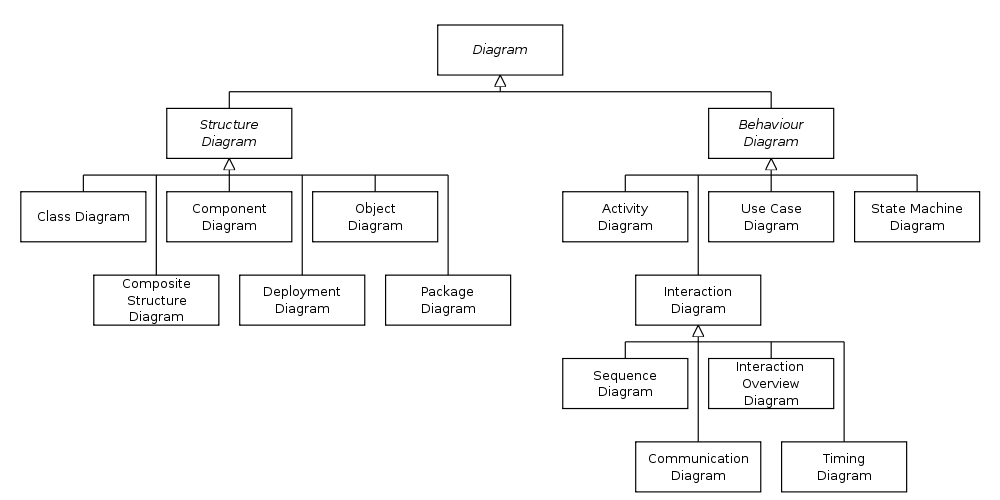
\includegraphics[width=320px, height=200px]{images/uml-diagram.png}
\end{frame}

\section{Разработка на ООП програми с Java}
\begin{frame}{Създаване на обекти}
  \transdissolve
  \begin{itemize}
  \item Конструктор \pause
    \begin{itemize}
    \item специален метод, който създава обект от даден клас \pause
    \item обикновено в него се инициализират атрибутите на обекта \pause
    \end{itemize}
  \item Конструктора има същото име като името на класа \pause
  \item Обръщения към конструктора трябва да се предшествани от
    ключовата дума
    \textbf{new}
  \end{itemize}
\end{frame}

\begin{frame}[fragile]
  \frametitle{Създаване на обекти - пример}
  \transdissolve
\begin{lstlisting}
Date currentDate; //not initialized
currentDate = new Date(); //create a new date object
System.out.println(currentDate.toString());
anotherDate = currentDate; // a second referrence to the first date
\end{lstlisting}
\end{frame}

\begin{frame}{Променливи от референтен тип}
  \transdissolve
  \begin{itemize}
  \item Променливите \alert{НЕ} са обекти \pause
  \item Променливите \alert{НЕ} съдържат обект \pause
  \item Променливите \alert{съдържат само препратка(референция,
      адрес)} на обект \pause
  \item Няколко променливи могат да сочат към
    един обект \pause
  \item Променливите \alert{НЕ} са инициализирани с
    null по подразбиране
  \end{itemize}
\end{frame}

\begin{frame}{Класове от стандартната библиотека}
  \transdissolve
  \begin{itemize}
  \item java.util.Date -  представя дата
  \item java.util.Random - генератор на случайни числа
  \item java.util.Scanner - вход от поток
  \item java.lang.System - агрегатор на системни
    операции
  \item java.util.GregorianCalendar - представя дата по
    грегорианския(нашия) календар
  \end{itemize}
\end{frame}

\begin{frame}{Разработка на класа Person}
  \transdissolve
  \begin{itemize}
  \item Полета \pause
    \begin{itemize}
    \item име \pause
    \item фамилия \pause
    \item адрес \pause
    \item дата на раждане \pause
    \end{itemize}
  \item Конструктори \pause
  \item Методи \pause
    \begin{itemize}
    \item аксесори(getters)/мутатори(setters) \pause
    \item кажи нещо \pause
    \item отиди някъде
    \end{itemize}
  \end{itemize}
\end{frame}

\begin{frame}{Работа с няколко сорс файла}
  \transdissolve
  \begin{itemize}
  \item Java компилатора разбира
    зависимостите между класовете \pause
  \item Ако клас А зависи(използва) от клас Б, то компилацията на A ще
    доведе автоматично до компилацията и на Б \pause
    \begin{itemize}
    \item javac A.java \pause
    \end{itemize}
–  \item Вградена функционалност тип \textbf{make}
  \end{itemize}
\end{frame}

\begin{frame}{Изследване на класа Person}
  \transdissolve
  \begin{itemize}
  \item Всички полета са маркирани с
    модификатора за достъп \textbf{private} \pause
  \item private ограничава достъпа до полетата
    само до рамките на класа, в който те са
    дефинирани \pause
  \item Осигурява се отлична капсулация на
    данните и достъпа до тях се контролира
    надеждно чрез методи
  \end{itemize}
\end{frame}

\begin{frame}{Изследване на класа Person}
  \transdissolve
  \begin{itemize}
  \item Всички методи са маркирани с
    модификатора за достъп \textbf{public} \pause
  \item public маркира програмен елемент като
    достъпен за ВСИЧКИ класове \pause
  \item Почти никога не е добра идея полета да
    бъдат маркирани като public - това
    нарушава капсулацията на данните
    основен принцип на ООП
    \begin{itemize}
      \item Изключение от това правило са константите и singleton обектите
    \end{itemize}
  \end{itemize}
\end{frame}

\begin{frame}{Представяне на обект като низ}
  \transdissolve
  \begin{itemize}
  \item Полезна техника за търсене на грешки \pause
  \item Метод toString() \pause
  \item Генериране на метода toString() в IntelliJ IDEA
  \end{itemize}
\end{frame}

\begin{frame}{Конструктор}
  \transdissolve
  \begin{itemize}
  \item има същото име като класа \pause
  \item Не връща резултат \pause
  \item Клас може да има повече от един
    конструктор \pause
  \item Конструктора може да приема различен
    брой аргументи \pause
  \item Конструктора може да бъде извикан
    само с ключовата дума \textbf{new}
  \end{itemize}
\end{frame}

\begin{frame}{Параметри на конструкторите}
  \transdissolve
  \begin{itemize}
  \item Преки
    \begin{itemize}
    \item стойността им се
      използва директно за инициализиране
      на поле
    \end{itemize}
  \item Непреки
    \begin{itemize}
    \item стойността им се
      използва като база за изчисляването на
      стойността, която да се зададе на поле
    \item например можем да използваме параметър дата на раждане за
      изчисляване на стойността на поле възраст
    \end{itemize}– 
  \item Препоръчително е конструкторът да няма повече от 4 параметъра
  \end{itemize}
\end{frame}

\begin{frame}{Предимства на енкапсулацията}
  \transdissolve
  \begin{itemize}
  \item Валидиране на данни \pause
  \item Защитаване на данни от промени \pause
  \item Гъвкавост - възможно е да бъде
    променена вътрешна имплементация
    без промени на публичното API
  \end{itemize}
\end{frame}

\begin{frame}[fragile]
  \frametitle{Допълнение за private}
  \transdissolve
  \begin{itemize}
  \item private членовете от всеки обект на
    класа са достъпни в неговите методи.
  \end{itemize}
\begin{lstlisting}
class Person {
  public int compare(Person another) {
    if (this.name.equals(another.name)) ...
  }
}
\end{lstlisting}
\end{frame}

\begin{frame}{Добрият стил диктува...}
  \transdissolve
  ... Само методите, които ще бъдат
  използвани от клиентски код да бъдат
  декларирани публични –
  допълнителните(utility) методи е
  желателно да бъдат private
\end{frame}

\begin{frame}{Модификатора final}
  \transdissolve
  \begin{itemize}
  \item Приложен към примитивен тип
    \begin{itemize}
      \item константа \pause
    \end{itemize}
  \item Приложен към обект
    \begin{itemize}
    \item константна референция, самия обект
      може да бъде променен \pause
    \end{itemize}
  \item Приложен към клас
    \begin{itemize}
    \item ненаследим клас \pause
    \end{itemize}
  \item Приложен към метод
    \begin{itemize}
    \item метод, който не
      може да бъде overridden
    \end{itemize}

  \end{itemize}
\end{frame}

\begin{frame}{Статични(класови) полета и методи}
  \transdissolve
  \begin{itemize}
  \item Асоциирани са съм самия клас, а не
    обектите инстанцирани от него \pause
  \item Достъпни са както посредством класа,
    така и посредство обектите от него \pause
  \item Статични полета често се използват за
    съхранение на константи \pause
  \item Статични методи често се използват за
    реализация на фабрични методи
  \end{itemize}
\end{frame}

\begin{frame}{Параметри на методите}
  \transdissolve
  \begin{itemize}
  \item Винаги се предават по стойност(by value)
    \begin{itemize}
    \item При примитивните типове се предава самата стойност на
      аргумента
    \item При референтните типове се предава препратка(адрес) към
      обекта. Самата препратка е непроменима, но обектът указан от
      нея е.
    \end{itemize}
  \item Прототип на метод - името и параметрите на метода, но не и
    връщаната му стойност
  \end{itemize}
\end{frame}

\begin{frame}{Конструиране на обекти}
  \transdissolve
  \begin{itemize}
  \item Обекти обикновено се създават посредством конструктор \pause
  \item Конструктор по подразбиране
    \begin{itemize}
      \item генериран автоматично от компилатора, ако няма изрично
        дефинирани конструктори
      \item не приема параметри
      \item изрично дефиниран конструктор, който не приема параметри
        \alert{НЕ} е конструктор по подразбиране
    \end{itemize}
 \pause
  \item Всички полета се инициализират със стойност по подразбиране
    \begin{itemize}
    \item 0 за числени типове
    \item null за референтни типове
    \item false за булеви полета
    \end{itemize} \pause
  \item Може да имате повече от един конструктор \pause
  \item Може да извиквате един конструктор от друг
  \end{itemize}
\end{frame}

\begin{frame}{Презареждане(overloading) на методи}
  \transdissolve
  \begin{itemize}
  \item Може да дефинирате няколко метода с едно и също име в даден
    клас стига сигнатурата им да е различна \pause
  \item Компилаторът използва сигнатурата, за да определи правилният
    метод, който да бъде извикан \pause
  \item Сигнатура(прототип)
    \begin{itemize}
    \item формални параметри
    \item име на метода
    \item \alert{НЕ} включва типа на връщаната от метода стойност
    \end{itemize}
  \end{itemize}
\end{frame}

\begin{frame}[fragile]
  \frametitle{Пример - презареждане}
  \transdissolve
\begin{lstlisting}
public class DataArtist {
  ...
  public void draw(String s) {...}
  public void draw(int i) {...}
  public void draw(double f) {...}
  public void draw(int i, double f) {...}
}
\end{lstlisting}
\end{frame}


\begin{frame}{Съвети за работа с конструктори}
  \transdissolve
  \begin{itemize}
  \item Именуване на параметрите \pause
  \item Навързване на конструктори \pause
  \item Конструктори с повече от 4-5 параметъра могат да бъдат
    заменени с шаблона за дизайн Builder \pause
  \item Конструкторите могат да бъдат заменени със статични
    методи-фабрика, които вътрешно използват private конструктори
  \end{itemize}
\end{frame}

\section{Организация и документация на класове}
\subsection{Пакети}
\begin{frame}{Пакети в Java}
  \transdissolve
  \begin{itemize}
  \item позволяват групиране на свързани класове \pause
  \item предотвратяват конфликти в имената на класове - приблизителен
    еквивалент на namespaces в C++/Java \pause
  \item съществува строга връзка между имената нивата в имената на
    пакетите съответстват на директории във файловата система \pause
  \item желателно е да са уникални - конвенцията диктува да започват
    обърнат наопаки домейнът на вашата организация \pause
  \item запазени имена на пакети - java.*, javax.*
  \end{itemize}
\end{frame}

\begin{frame}{Импортиране на класове и пакети}
  \transdissolve
  \begin{itemize}
  \item Всеки клас има достъп до всички класове в неговия пакет без
    допълнителни импорти \pause
  \item Всеки клас има достъп до всички публични класове, които са
    импортирани или използвани с напълно квалифицирани имена \pause
  \item Всички класове от един пакет могат да бъдат импортирани с
    wildcard import(*), но това не е препоръчително
  \end{itemize}
\end{frame}

\begin{frame}{Статични импорти}
  \transdissolve
  \begin{itemize}
  \item Импортиране само на определени статични елементи от даден клас
    - полета или методи \pause
  \item Подходяща техника за работа със статични класове като
    java.util.Math \pause
  \item Могат да нарушат четимостта на програмата, ако се използват безразборно
  \end{itemize}
\end{frame}

\begin{frame}{Особености на пакетите}
  \transdissolve
  \begin{itemize}
  \item Всяка част от името на пакета е отделена от другите с точка и
    съответства на поддиректория в директорията с кода
    \begin{itemize}
    \item пакет - bg.drow.spellbook
    \item директория bg/drow/spellbook
    \end{itemize}
  \item Не съществува йерархична организация на пакетите
  \end{itemize}
\end{frame}

\subsection{Разпространение на Java код}
\begin{frame}{Пакетиране на Java код}
  \transdissolve
  \begin{itemize}
  \item jar архив
    \begin{itemize}
    \item bytecode + мета информация, компресирани със zip
    \end{itemize} \pause
  \item Добавяне на jar архиви в клас пътя на виртуалната машина \pause
  \item Изпълнение на код пакетиран в jar архив
    \begin{itemize}
    \item java -jar somejar.jar MainClass
    \end{itemize}
  \end{itemize}
\end{frame}

\begin{frame}{Java Classpath}
  \transdissolve
  \begin{itemize}
  \item Указва местата, където виртуалната машина търси класове, при
    изпълнението на дадена програма \pause
  \item може да се задава като параметър от командния ред или като
    настройка на средата \pause
  \item Източник на много проблеми
  \end{itemize}
\end{frame}

\begin{frame}{Пример}
  \transdissolve
  \begin{itemize}
  \item В UNIX(Linux, Solaris, BSD)
      \begin{itemize}
      \item java -cp .:dir2:dir3 MyClass
      \item export CLASSPATH=.:dir2:dir3
      \end{itemize} \pause
    \item В Windows:
      \begin{itemize}
      \item Java -cp .;dir2;dir3; MyClass
      \item set CLASSPATH=.;dir2;dir3
      \end{itemize}
  \end{itemize}
\end{frame}

\subsection{Документиране на код}
\begin{frame}{Документиране на класове с javadoc}
  \transdissolve
  \begin{itemize}
  \item Разглеждане на javadoc документация
  \item Документира се само публичния интерфейс на едно API
  \item Стандартни javadoc анотации
  \item Работа с инструмента javadoc
  \end{itemize}
\end{frame}

\begin{frame}{Работа с javadoc}
  \transdissolve
  \begin{itemize}
  \item Документиране на един пакет
    \begin{itemize}
    \item javadoc -d docdir package
    \end{itemize}
  \item създава документация за няколко пакета
    \begin{itemize}
    \item javadoc -d docdir package1, package2
    \end{itemize}
  \end{itemize}
\end{frame}

\begin{frame}{Седем прости правила за създаване на добри класове}
  \transdissolve
  \begin{enumerate}
  \item Правете всички полета private \pause
  \item Инициализирайте изрично всички полета \pause
  \item Не използвайте много примитивни полета \pause
  \item Не слагайте get/set методи, ако нямате нужда от тях \pause
  \item Дефинирайте класовете по стандартен начин \pause
  \item Раздробявайте класовете с много отговорности на по-малки \pause
  \item Избирайте смислени име за класовете, полетата и методите
  \end{enumerate}
\end{frame}

\begin{frame}{Упражнение}
  \transdissolve
  \begin{itemize}
    \item Реализирайте клас Rational, който представя дроби и
      предоставя математически операции за работа с тях - събиране,
      изваждане, умножение и делене. Всички негови методи, трябва да
      могат да работят освен с други дроби и с цели числа.
  \end{itemize}
\end{frame}

\section*{Заключение}

\begin{frame}{Заключение}
  \transdissolve
  % Keep the summary *very short*.
  \begin{itemize}
  \item
    Класовете са шаблоните, по които изграждаме обекти.
  \item
    Обектите са градивните блокове на типичната Java програма.
  \item
    Проектирането на класове е критичен процес, при който трябва да
    бъдат съблюдавани утвърдените практики.
  \end{itemize}
  
  % The following outlook is optional.
  \vskip0pt plus.5fill
  \begin{itemize}
  \item
    Следващият път:
    \begin{itemize}
    \item
      Наследяване
    \item
      Полиморфизъм
    \end{itemize}
  \end{itemize}
\end{frame}

\begin{frame}{Въпроси}
  \transdissolve
  \begin{center}
    \LARGEТук е момента да зададете вашите въпроси! :-)
  \end{center}
\end{frame}

\begin{frame}{Край}
  \transdissolve
  \begin{center}
    \LARGEБлагодаря Ви за вниманието!
  \end{center}
\end{frame}

\end{document}

%%% Local Variables: 
%%% mode: latex
%%% TeX-master: t
%%% End: 
